\chapter{軸対称円盤の質量積分と回転曲線}
\label{app:disk-integrals}

第1章では、球対称な密度分布から内包質量を求め、数値積分法の精度を検証した。
本付録では、Ryden §6.5 の薄い軸対称円盤を題材として、既習の数値積分を別の問題へ適用する\cite{ryden2025}。
球殻から円環へ質量要素を変え、同じ累積台形則で指数円盤の内包質量を求める。
解析解との比較と格子収束試験によって、実装を再利用した場合も精度を確かめる。

後半では、円盤の回転曲線と球対称近似を比較する。
ここでは解析式を用い、数値積分の誤差を混ぜずに、質量分布の仮定による違いを調べる。
数値手法を再利用できることと、物理の関係式をそのまま使えることは別である。
本付録は第1章の発展内容であり、第2・3章や他の付録を先に読む必要はない。

\begin{learningbox}[本付録で学ぶこと]
\begin{itemize}
\item 軸対称円盤の質量を求める問題について、数値積分の被積分関数と積分区間を設定できる。
\item 被積分関数を入れ替え、第1章の累積台形則の実装を別の質量分布に再利用できる。
\item 解析解との比較と格子収束試験から、累積積分の誤差と収束次数を評価できる。
\item 数値積分の離散化誤差と、有限の計算領域の外にある質量を区別できる。
\item 数値計算の誤差と、物理モデルの仮定によって生じる違いを区別できる。
\end{itemize}
\end{learningbox}

数値実験は Notebook A で行う。
積分公式と累積積分の実装には、第1章で学んだものを使う\cite{kouya2021}。
本文では、被積分関数の設定、既習の実装の使い方、数値結果の検証を説明する。

\section{球対称系と軸対称円盤の質量要素}
\label{sec:appA-annulus}

球対称系では、半径 $r$、厚さ $dr$ の球殻の質量は
\begin{equation}
 dM=4\pi r^2\rho(r)\,dr
\end{equation}
であった。
一方、無限に薄い軸対称円盤では、円盤面内で中心から測った半径を $R$ とし、単位面積あたりの質量を\textbf{面密度（surface density）} $\Sigma(R)$ で表す。
半径 $R$、幅 $dR$ の薄い\textbf{円環（annulus）}の面積は、円周に幅を掛けた
\begin{equation}
 dA=2\pi R\,dR
\end{equation}
なので、その質量は
\begin{equation}
 dM=2\pi R\Sigma(R)\,dR
\label{eq:appA-annulus-mass}
\end{equation}
となる。半径 $R$ より内側の内包質量は
\begin{equation}
 \boxed{M(<R)=\int_0^R 2\pi R'\Sigma(R')\,dR'.}
\label{eq:appA-enclosed-integral}
\end{equation}
ここで $R'$ は積分変数である。
数値積分に渡す被積分関数は $\Sigma(R')$ そのものではなく、$2\pi R'\Sigma(R')$、積分区間は $[0,R]$ である。
球対称系の $4\pi r'^2\rho(r')$ をこの関数に入れ替えれば、同じ1次元の積分法を使える。

\section{指数円盤の内包質量}
\label{sec:appA-exponential}

数値積分の検証には、内包質量を解析的に求められる\textbf{指数円盤（exponential disk）}
\begin{equation}
 \Sigma(R)=\Sigma_0 e^{-R/R_d}
\label{eq:appA-surface-density}
\end{equation}
を使う。
$\Sigma_0$ は中心面密度、$R_d$ は面密度が中心値の $1/e$ になる半径である\cite{ryden2025}。

\subsection{全質量と中心面密度}

円盤の全質量を $M_d$ とすると、式\eqref{eq:appA-enclosed-integral}の上端を無限大にして
\begin{equation}
 M_d=2\pi\Sigma_0\int_0^\infty R'e^{-R'/R_d}\,dR'
\end{equation}
である。
$u=R'/R_d$ と変数変換すれば、$R'=R_du$、$dR'=R_d\,du$ なので
\begin{equation}
 M_d=2\pi\Sigma_0R_d^2\int_0^\infty ue^{-u}\,du.
\end{equation}
部分積分から
\begin{equation}
 \int ue^{-u}\,du=-ue^{-u}+\int e^{-u}\,du=-(u+1)e^{-u}+C
\label{eq:appA-antiderivative}
\end{equation}
となる。$C$ は積分定数である。
上端と下端で評価すると定積分の値は1なので、
\begin{equation}
 M_d=2\pi\Sigma_0R_d^2,\qquad \Sigma_0=\frac{M_d}{2\pi R_d^2}
\label{eq:appA-normalization}
\end{equation}
を得る。Notebook A では $M_d$ と $R_d$ を指定して $\Sigma_0$ を決める。

\subsection{有限半径までの内包質量}

同じ変数変換を有限の上端 $R$ に対して使うと、
\begin{align}
 M(<R)&=2\pi\Sigma_0R_d^2\int_0^{R/R_d}ue^{-u}\,du\notag\\
 &=M_d\left[1-e^{-R/R_d}\left(1+\frac{R}{R_d}\right)\right]
\label{eq:appA-mass-exact}
\end{align}
となる。
式\eqref{eq:appA-antiderivative}を上端と下端で評価し、式\eqref{eq:appA-normalization}を使った。
これは Ryden の式(6.161)に対応する解析解であり、$R=0$ で0、$R\to\infty$ で $M_d$ となる\cite{ryden2025}。
以下では、この式を有限半径までの数値積分を検証する基準にする。

\subsection{被積分関数と実装}

被積分関数は
\begin{equation}
 f_M(R)\equiv\frac{dM}{dR}=2\pi R\Sigma(R)=\frac{M_d}{R_d}\frac{R}{R_d}e^{-R/R_d}
\label{eq:appA-mass-integrand}
\end{equation}
である。
面密度は中心で最大だが、$f_M$ は $R=0$ で0になる。一定幅の円環の面積が中心へ向かって小さくなるためである。
図\ref{fig:appA-profiles}では、面密度と被積分関数をそれぞれの基準量で割り、半径に対する形を比較する。

\begin{figure}[!htbp]
\centering
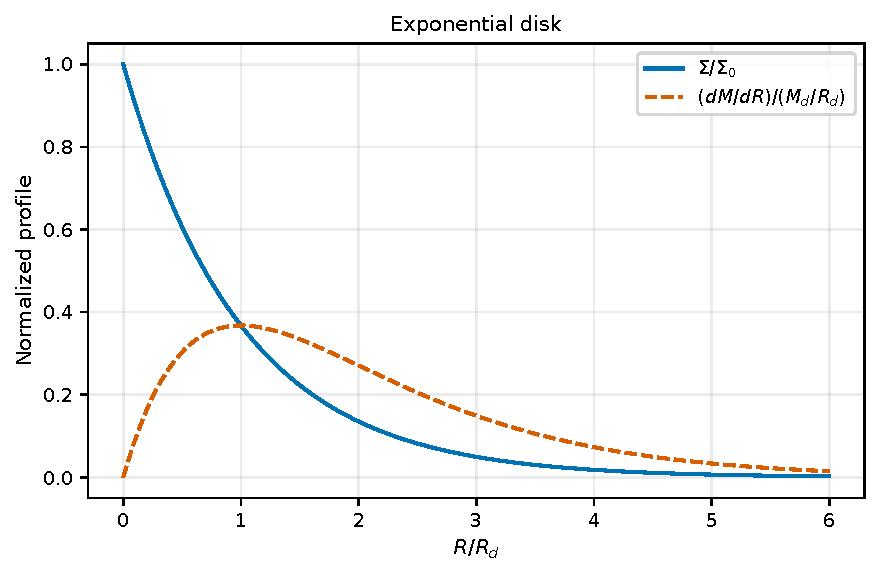
\includegraphics[width=0.64\linewidth]{appA_exponential_profiles.pdf}
\caption{指数円盤の面密度と、一定の動径幅あたりの質量。面密度は $\Sigma_0$、被積分関数 $dM/dR$ は $M_d/R_d$ で規格化した。両者は異なる物理量なので、ここでは半径に対する形の違いを比較する。}
\label{fig:appA-profiles}
\end{figure}

式\eqref{eq:appA-surface-density}と式\eqref{eq:appA-mass-integrand}を関数にすると、Listing A.1 になる。
\texttt{sigma\_exponential} が面密度、\texttt{dMdR\_exponential} が数値積分に渡す被積分関数を返す。

\begin{listingbox}{A.1　指数円盤の面密度と被積分関数}
\begin{Verbatim}[fontsize=\small]
def sigma_exponential(R, Md=1.0, Rd=1.0):
    Sigma0 = Md / (2.0 * np.pi * Rd**2)
    return Sigma0 * np.exp(-R / Rd)

def dMdR_exponential(R, Md=1.0, Rd=1.0):
    return 2.0 * np.pi * R * sigma_exponential(R, Md, Rd)
\end{Verbatim}
\end{listingbox}

\section{累積台形則による数値積分}
\label{sec:appA-cumulative}

計算領域 $0\le R\le R_{\max}$ を $N$ 個の区間に分け、
\begin{equation}
 R_i=i\Delta R,\qquad \Delta R=\frac{R_{\max}}{N},\qquad i=0,1,\ldots,N
\label{eq:appA-grid}
\end{equation}
とする。
第1章の累積台形則を $f_M$ に使えば、内包質量の数値近似 $M_i\simeq M(<R_i)$ は
\begin{equation}
 M_0=0,\qquad M_{i+1}=M_i+\frac{\Delta R}{2}\left[f_M(R_i)+f_M(R_{i+1})\right]
\label{eq:appA-cumulative-trapezoid}
\end{equation}
で求められる。$i=0,1,\ldots,N-1$ の順に更新すれば、各半径について0から積分をやり直す必要はない。

実装には第1章の Listing 1.5 の \texttt{cumulative\_trapezoid\_manual} を使う。
この関数は、引数 \texttt{x} に格子、\texttt{y} に被積分関数の値を受け取り、各区間の台形面積を \texttt{np.cumsum} で累積する。
ここでは \texttt{x} に $R_i$、\texttt{y} に $f_M(R_i)$ を渡す。
積分する関数が変わるだけで、累積加算の実装は変わらない（\S\ref{sec:ch1-cumulative}）。

\begin{notebookblock}{A｜内包質量の数値積分}
$G=M_d=R_d=1$ とし、$0\le R\le10R_d$ を400区間に分ける。
\texttt{R} は両端を含む401個の格子点である。
\texttt{mass\_exponential\_exact} は式\eqref{eq:appA-mass-exact}を返す関数で、完全な定義は Notebook A に置く。

{\sffamily\small\color{graytext}対応セル（計算部分）}
\begin{Verbatim}[xleftmargin=2mm,fontsize=\small,frame=single,framesep=1.8mm,framerule=0.35pt,rulecolor=\color{listingframe},fillcolor=\color{listingbg}]
# 0 <= R <= 10 Rd を N=400 区間に分ける
N = 400
R_max = 10.0 * Rd
R = np.linspace(0.0, R_max, N + 1)

# 被積分関数 dM/dR = 2 pi R Sigma(R) を格子点で評価する
dMdR = dMdR_exponential(R, Md, Rd)

# 累積台形則と、同じ格子点での解析解を比較する
M_num = cumulative_trapezoid_manual(R, dMdR)
M_exact = mass_exponential_exact(R, Md, Rd)

# 積分誤差と、計算領域の外にある質量を別々に測る
mass_error_outer = (M_num[-1] - M_exact[-1]) / Md
mass_outside = (Md - M_exact[-1]) / Md
\end{Verbatim}
\end{notebookblock}

同じ格子点で得た数値解と解析解を図\ref{fig:appA-mass-profile}に示す。
二つの曲線はほぼ重なり、外側の格子点では
\begin{equation}
 \frac{M_{\rm num}(<R_{\max})}{M_d}=\appAMassRmaxNum,\qquad
 \frac{M_{\rm exact}(<R_{\max})}{M_d}=\appAMassRmaxExact
\label{eq:appA-mass-at-rmax}
\end{equation}
となる。
両者の差が、同じ上端まで積分したときの数値積分の誤差である。

\begin{figure}[!htbp]
\centering
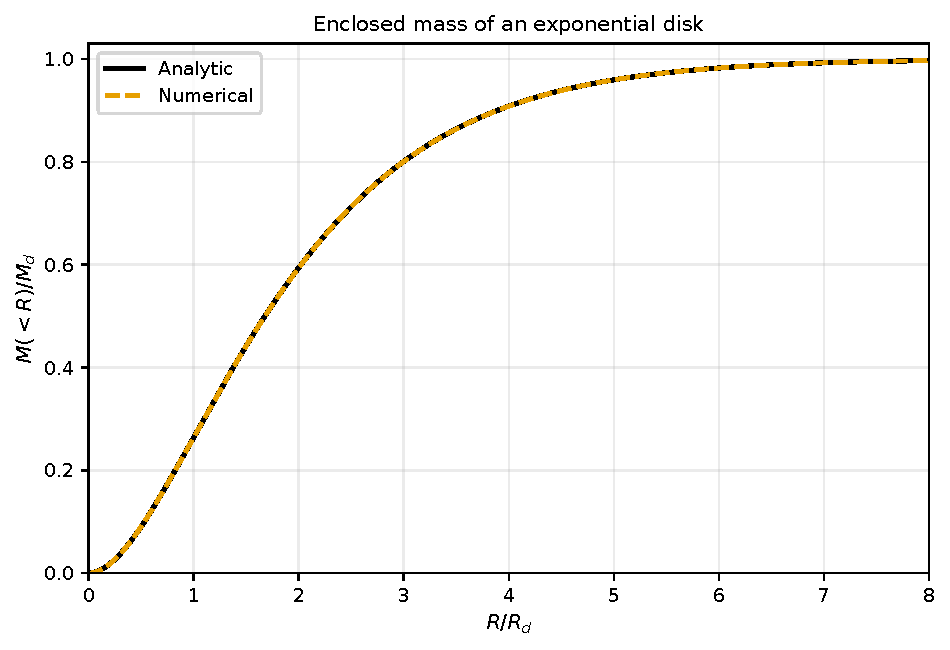
\includegraphics[width=0.64\linewidth]{appA_mass_profile.pdf}
\caption{指数円盤の内包質量の解析解と累積台形積分。計算は $0\le R\le10R_d$ を400区間に分けて行い、図には $R\le8R_d$ の範囲を示す。質量は円盤の全質量 $M_d$ で規格化している。}
\label{fig:appA-mass-profile}
\end{figure}

\subsection{積分誤差と計算領域の外にある質量}

一方、解析解でも $M_{\rm exact}(<R_{\max})<M_d$ である。
その差は数値積分の誤差ではなく、計算領域の外にある質量であり、式\eqref{eq:appA-mass-exact}から
\begin{equation}
 \frac{M_d-M_{\rm exact}(<R_{\max})}{M_d}
 =e^{-R_{\max}/R_d}\left(1+\frac{R_{\max}}{R_d}\right)
\label{eq:appA-mass-outside}
\end{equation}
と求められる。
$R_{\max}$ を固定したまま格子を細かくすると、数値解はその上端までの解析解へ近づくが、領域外の質量は変わらない。
全質量 $M_d$ を有限半径までの積分で近似する場合には、積分の離散化誤差とは別に、この寄与も考える必要がある。

\section{累積台形則の格子収束}
\label{sec:appA-convergence}

一つの格子で解析解と重なるだけでは、誤差が期待した次数で減るかは分からない。
計算領域を $R_{\max}=10R_d$ に固定し、全格子点での誤差を
\begin{equation}
 \epsilon_M\equiv\max_{0\le i\le N}\frac{|M_{\rm num}(<R_i)-M_{\rm exact}(<R_i)|}{M_d}
\label{eq:appA-mass-error}
\end{equation}
で測る。
これは全質量 $M_d$ で規格化した最大絶対誤差であり、各点の内包質量に対する相対誤差ではない。
一定の $M_d$ を分母に使うことで、内包質量が0の中心も評価に含められる。

第1章で学んだ台形則の誤差評価から、滑らかな被積分関数を固定区間で積分すると、離散化誤差が支配する範囲では
\begin{equation}
 \epsilon_M\simeq C\left(\frac{\Delta R}{R_d}\right)^p,\qquad p=2
\label{eq:appA-convergence-law}
\end{equation}
が期待される。ここで $C$ は格子幅によらない係数である。
累積積分でも、各上端まで同じ台形則で積分するため、この誤差評価を使える。
$R_d$ を固定しているので、$\log\Delta R$ に対する $\log\epsilon_M$ の傾きも $p$ となる。

\noindent\textbf{検証手順｜累積台形則の格子収束}
\begin{enumerate}
\item 計算領域と $M_d,R_d$ を固定し、区間数を $N=25,50,100,200,400,800$ と変える。
\item 各格子で累積積分と解析解を比較し、式\eqref{eq:appA-mass-error}の最大誤差を測る。
\item 両対数で誤差が規則的に減少する範囲を確かめ、その傾きを2と比較する。
\end{enumerate}

\begin{notebookblock}{A｜累積台形則の格子収束}
\texttt{exponential\_mass\_error} は1つの格子の幅と最大誤差を返す。
区間数を2倍ずつ増やし、格子幅を半分にして計算を繰り返す。

{\sffamily\small\color{graytext}対応セル（計算部分）}
\begin{Verbatim}[xleftmargin=2mm,fontsize=\footnotesize,frame=single,framesep=1.8mm,framerule=0.35pt,rulecolor=\color{listingframe},fillcolor=\color{listingbg}]
# 1つの格子で内包質量の最大誤差を測る
def exponential_mass_error(N, R_max=10.0, Md=1.0, Rd=1.0):
    R = np.linspace(0.0, R_max, N + 1)
    dMdR = dMdR_exponential(R, Md, Rd)
    M_num = cumulative_trapezoid_manual(R, dMdR)
    M_exact = mass_exponential_exact(R, Md, Rd)
    dR = R[1] - R[0]
    err = np.max(np.abs(M_num - M_exact)) / Md
    return dR, err

# 領域とモデルを固定し、区間数を2倍ずつ増やす
N_values = np.array([25, 50, 100, 200, 400, 800])
dR_values = []
mass_errors = []
for N_i in N_values:
    dR_i, err_i = exponential_mass_error(int(N_i), 10.0 * Rd, Md, Rd)
    dR_values.append(dR_i)
    mass_errors.append(err_i)

dR_values = np.array(dR_values)
mass_errors = np.array(mass_errors)

# log(error)-log(dR) の直線の傾きが収束次数 p
order_mass = np.polyfit(np.log(dR_values), np.log(mass_errors), 1)[0]
\end{Verbatim}
\end{notebookblock}

図\ref{fig:appA-mass-convergence}では、6格子の誤差がほぼ2次の傾きで減少している。
これらすべての点を両対数で直線近似すると、
\begin{equation}
 p=\appAMassOrder
\label{eq:appA-mass-order}
\end{equation}
を得る。
球対称系から円盤へ題材を変えても、累積台形則の約2次の収束を確認できる。
格子をさらに細かくする場合も、当てはめには離散化誤差が規則的に減少する範囲を使い、丸め誤差で停滞した点や誤差が0の点は含めない。

\begin{figure}[!htbp]
\centering
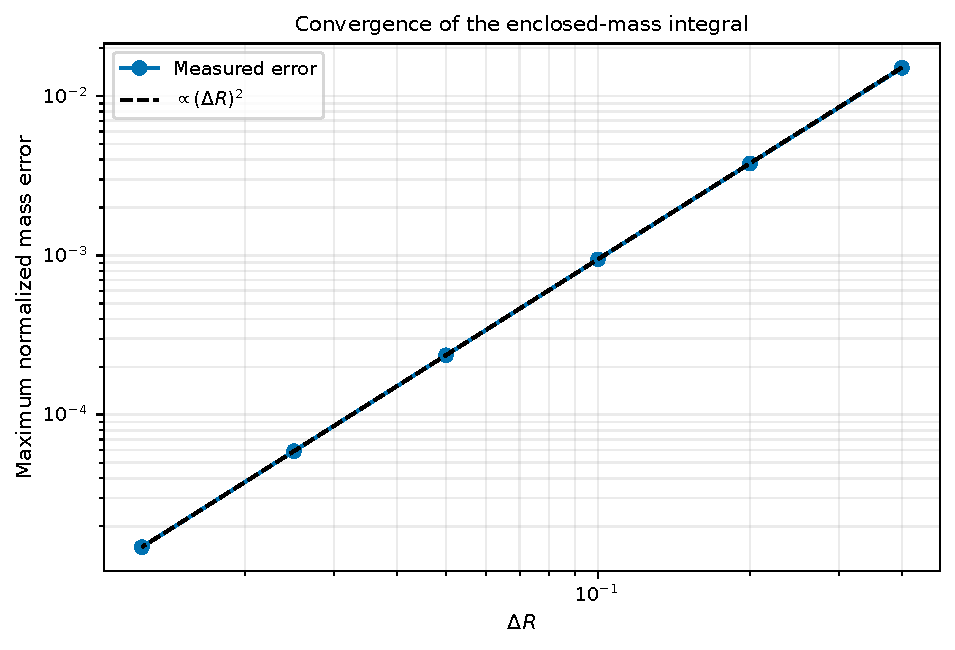
\includegraphics[width=0.64\linewidth]{appA_mass_convergence.pdf}
\caption{指数円盤の累積台形積分の格子収束。縦軸は式\eqref{eq:appA-mass-error}の誤差、横軸は $R_d=1$ の単位での格子幅である。破線は最も細かい格子での誤差を基準にした $(\Delta R)^2$ の線である。}
\label{fig:appA-mass-convergence}
\end{figure}

\section{指数円盤の回転曲線と球対称近似}
\label{sec:appA-rotation}

ここまでは、同じ積分問題に対する数値解と解析解の差を調べた。
次に、物理モデルの仮定によって結果がどう変わるかを見る。
第1章の球対称系では、Newton の球殻定理から
\begin{equation}
 v_{\rm circ}^2(r)=\frac{GM(<r)}{r}
\end{equation}
と書けた。
しかし円盤面内では、半径 $R$ より外側の質量も重力に寄与する。
球殻のように外側の質量の寄与が打ち消し合うわけではないため、その半径より内側の総質量だけでは円運動速度を決められない。

薄い指数円盤の回転曲線は、\textbf{修正 Bessel 関数（modified Bessel functions）}を用いて
\begin{equation}
 v_{\rm disk}^2(R)=4\pi G\Sigma_0R_d\,y^2\left[I_0(y)K_0(y)-I_1(y)K_1(y)\right],
 \qquad y=\frac{R}{2R_d}
\label{eq:appA-disk-rotation}
\end{equation}
と表せる。
$I_n$ と $K_n$ は、それぞれ第1種・第2種の $n$ 次修正 Bessel 関数であり、ここでは $n=0,1$ を使う。
この式は、Ryden の式(6.149)にある薄い円盤の Hankel 積分を指数円盤について評価した形に対応する。Ryden の図6.6には、その回転曲線が示されている\cite{ryden2025}。
本付録では式\eqref{eq:appA-disk-rotation}の導出には立ち入らず、比較に使う解析式として扱う。
Notebook A では \texttt{scipy.special.iv} と \texttt{kv} で関数値を求める。Hankel 積分を直接数値積分する方法は本書では扱わない。

比較曲線は、同じ内包質量を球対称分布のものとみなして
\begin{equation}
 v_{\rm sph}^2(R)\equiv\frac{GM_{\rm exact}(<R)}{R}
\label{eq:appA-spherical-comparison}
\end{equation}
と定義する。
内包質量には数値積分値ではなく解析解を使い、累積台形則の誤差を比較に混ぜない。
二つの曲線の違いは、数値積分法ではなく、質量分布を球対称とみなすことによって生じる。

\begin{notebookblock}{A｜指数円盤と球対称近似の比較}
$10^{-4}R_d\le R\le6R_d$ に等間隔の4000点を置き、二つの解析式を同じ半径で評価する。
\texttt{np.argmax} で、それぞれの最大値をとる格子点を選ぶ。作図と出力の整形は Notebook A に置く。

{\sffamily\small\color{graytext}対応セル（計算部分）}
\begin{Verbatim}[xleftmargin=2mm,fontsize=\footnotesize,frame=single,framesep=1.8mm,framerule=0.35pt,rulecolor=\color{listingframe},fillcolor=\color{listingbg}]
from scipy.special import iv, kv

# 回転曲線を評価する半径と y = R/(2 Rd)
R_rot = np.linspace(1.0e-4 * Rd, 6.0 * Rd, 4000)
y = R_rot / (2.0 * Rd)

# 修正 Bessel 関数による解析式を評価する
Bessel_term = iv(0, y) * kv(0, y) - iv(1, y) * kv(1, y)
vc2_disk = 4.0 * np.pi * G * Sigma0 * Rd * y**2 * Bessel_term

# 解析的な内包質量から球対称の比較曲線を作る
M_rot = mass_exponential_exact(R_rot, Md, Rd)
vc2_sph = G * M_rot / R_rot

# それぞれの最大値をとる格子点を求める
i_disk = np.argmax(vc2_disk)
i_sph = np.argmax(vc2_sph)
Rpeak_disk = R_rot[i_disk]
Rpeak_sph = R_rot[i_sph]
vc2peak_disk = vc2_disk[i_disk]
vc2peak_sph = vc2_sph[i_sph]
\end{Verbatim}
\end{notebookblock}

表\ref{tab:appA-rotation-peaks}に結果を示す。
$R_{\rm peak}$ は最大値をとる格子点の半径、$v_{\rm peak}$ はそこでの円運動速度である。
補間や最適化によって連続的な最大位置を求めた値ではない。
球対称近似では、最大位置が内側へずれ、最大速度も小さくなる。

\begin{table}[!htbp]
\centering
\caption{指数円盤の回転曲線と、同じ内包質量を用いた球対称近似の比較。速度の二乗は $GM_d/R_d$ で規格化している。}
\label{tab:appA-rotation-peaks}
\begin{tabular}{lcc}
\toprule
重力場のモデル & $R_{\rm peak}/R_d$ & $v_{\rm peak}^2/(GM_d/R_d)$\\
\midrule
指数円盤 & $\appADiskPeakR$ & $\appADiskPeakVTwo$\\
球対称近似 & $\appASphPeakR$ & $\appASphPeakVTwo$\\
\bottomrule
\end{tabular}
\end{table}

この違いは、回転曲線を評価する点を増やしてもなくならない。
数値積分が高い精度でできることと、物理の関係式が対象に適用できることは、分けて判断する必要がある。
図\ref{fig:appA-rotation}の実線と破線は、両曲線を共通の値 $v_{\rm max,disk}^2$ で割って示す。各曲線をそれぞれの最大値で割ったものではないので、振幅の違いも比較できる。

\section{Mestel 円盤と平坦な回転曲線}
\label{sec:appA-mestel}

一つのモデルで関係式が成り立っても、他のモデルで使えるとは限らない。
面密度が $\Sigma(R)\propto1/R$ の Mestel 円盤では、$2\pi R\Sigma(R)$ が一定なので、
\begin{equation}
 M(<R)\propto R,\qquad \frac{GM(<R)}{R}=\mathrm{const.}
\end{equation}
となる。
無限に広がる Mestel 円盤では、円盤の重力場から求めた円運動速度も一定であり、$v_{\rm circ}^2=GM(<R)/R$ が成立する。
ただし、これはこの分布に特有の結果であり、一般の円盤に使える関係ではない。

Ryden の式(6.150)では有限半径で打ち切ったモデルを導入し、式(6.158)--(6.159)で無限円盤との違いを説明している\cite{ryden2025}。
有限半径で打ち切ると、外側の質量の寄与が変わり、端の影響によって同じ等式は厳密には成り立たない。
本付録と Notebook A では有限 Mestel 円盤の重力場は計算せず、無限円盤の平坦な回転曲線を形の比較にだけ使う。

\begin{figure}[!htbp]
\centering
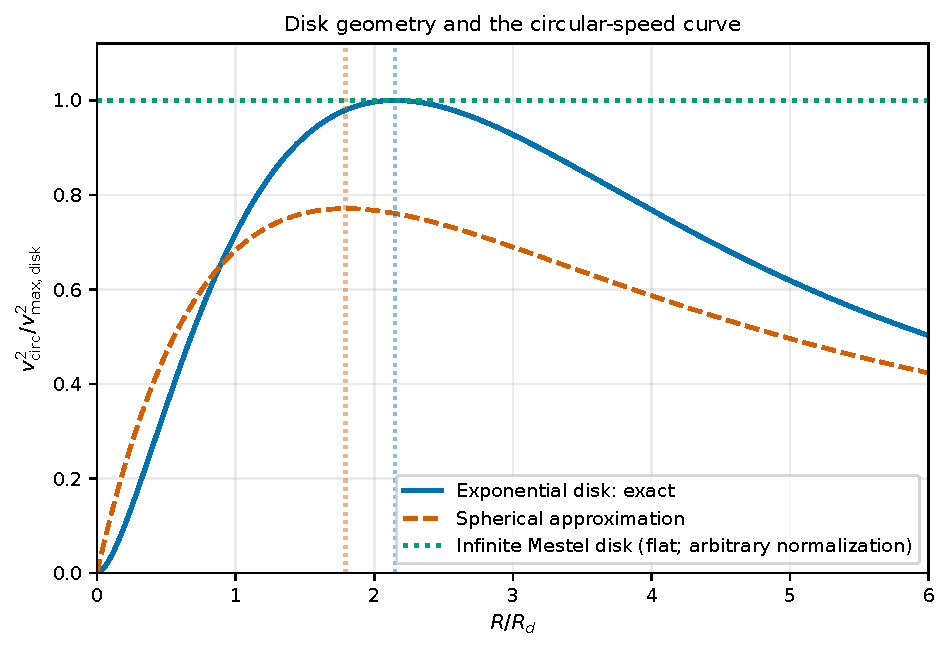
\includegraphics[width=0.69\linewidth]{appA_rotation_curve.pdf}
\caption{指数円盤の回転曲線と球対称近似。縦軸は速度の二乗を指数円盤の最大値 $v_{\rm max,disk}^2$ で割ったもので、表\ref{tab:appA-rotation-peaks}の規格化とは異なる。Mestel 円盤の点線は、無限円盤の平坦な形を示す任意規格化の線である。}
\label{fig:appA-rotation}
\end{figure}

\begin{cautionblock}{Mestel 円盤の比較線は任意規格化である}
図\ref{fig:appA-rotation}の点線は、指数円盤と同じ全質量や長さスケールから計算したものではない。
平坦な回転曲線の形を示すため、指数円盤の最大値に合わせている。
有限 Mestel 円盤の計算結果や、指数円盤と振幅まで物理的に対応する曲線として解釈してはいけない。
\end{cautionblock}

